\chapter{Understanding and Modeling the Physiological Environment}
\begin{itemize}
		\item How the device interacts with the environment?
		\item How much details should the environment models capture?
    \item What are the different modeling philosophies when developing environment models for different applications?
\end{itemize}

Medical devices are designed to interact with the human body aiming to improve physiological conditions of the patients. The knowledge of  the physiological context and how it can be changed by the devices is essential for 1) constructing physiological models; 2) understanding and encoding physiological requirements; 3) evaluating the closed-loop interactions between the human body and the devices. It is important to understand and model the physiological environment of the device at the level that 1) unnecessary details unrelated to the interaction between the device and the human are abstracted away, and 2) essential details required to differentiate different patient conditions are maintained.

Models (especially environment models) should be designed in accordance with their respective applications. During model-based development of medical devices, the environment model can be used for 1) closed-loop testing and 2) closed-loop model checking. Each application has different focus thus has very distinct requirements for the models. These requirements will affect the basic properties of the models, including 1) model complexity, 2) model identifiability etc. 

\textbf{Model Complexity} is generally measured in terms of the size of state space and/or computation complexity of state transitions, which affects the computation cost (memory and time) for closed-loop verification. The complexity requirements of an environment model is usually determined by 1) The complexity of the interactions between the environment model and the system model and 2) The complexity of the environment condition specified in the physiological requirements.

\textbf{Model Identifiability} is a metric of the feasibility/difficulty of identifying model parameters from data. It affects the validity of the model which is a key element for closed-loop verification. Model identifiability is generally affected by 1) Model complexity and 2) Data availability/quality. In general, the more complex the model structure is, the harder the model can be fully identified. For physiological modeling, the data availability is almost always an issue.


In the following sections, we introduce the physiological context that the pacemaker operates in, and how to construct heart models for closed-loop verification of implantable pacemaker. Note that for two different applications the models are constructed differently as we address their respective requirements for environment models. 
\begin{figure}[!t]
\centering
		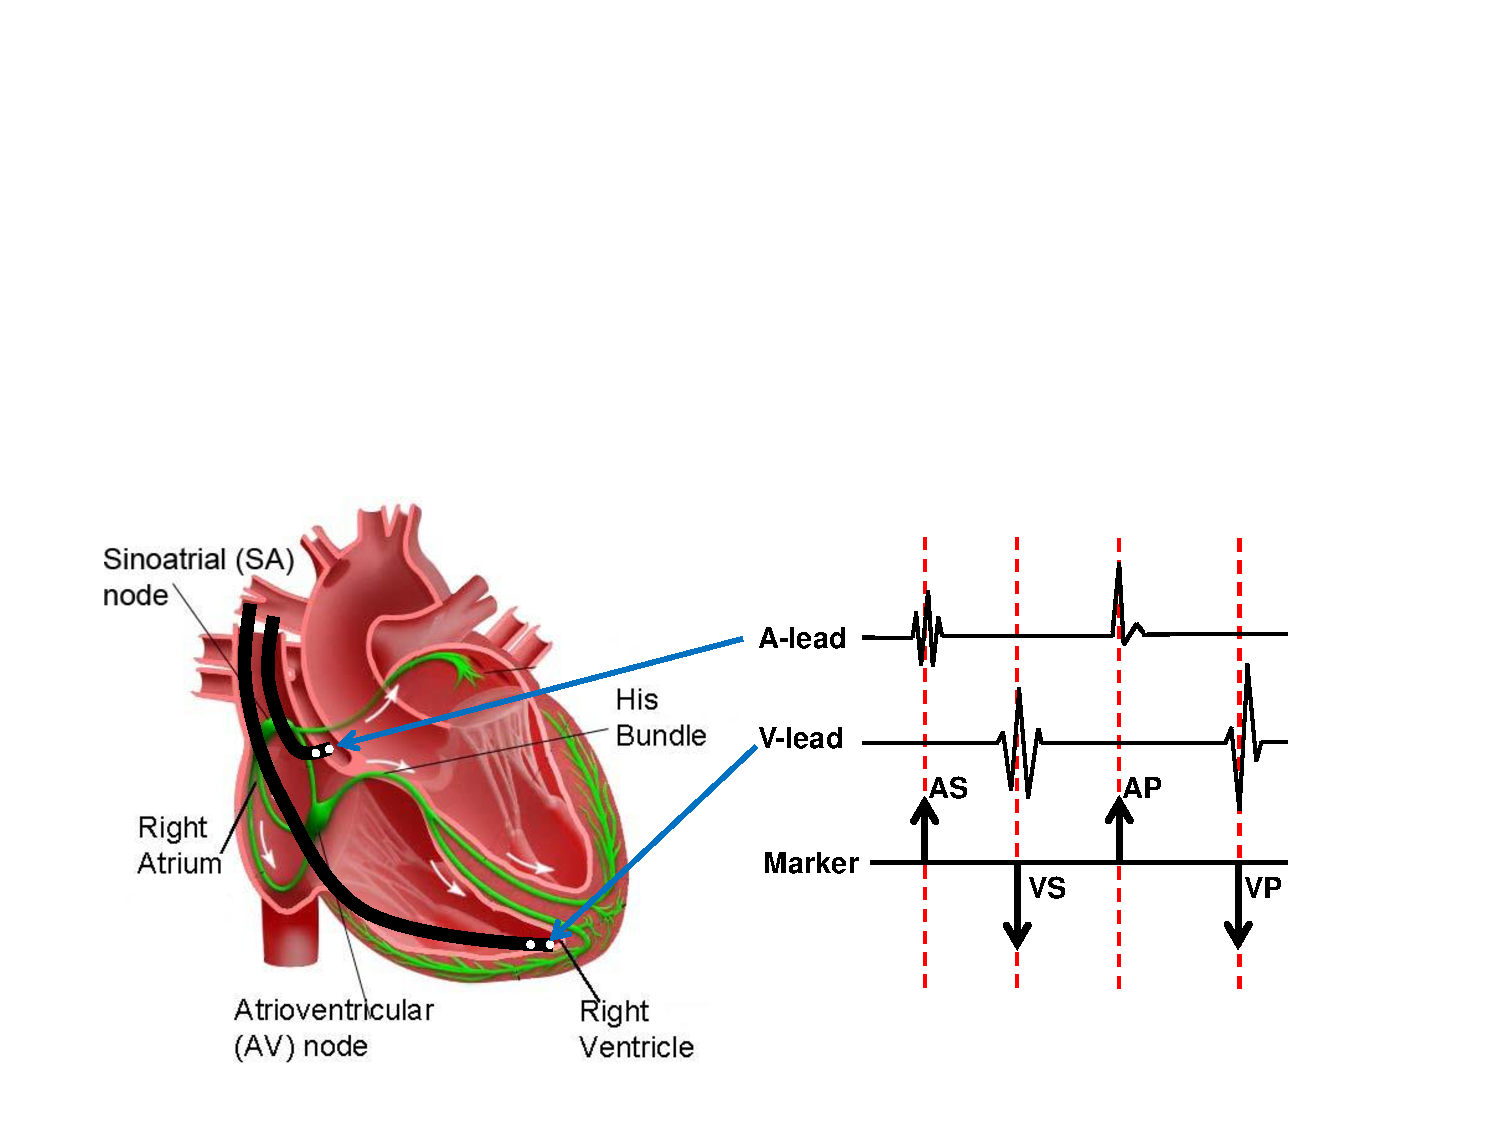
\includegraphics[width=0.9  \textwidth]{figs/egm.pdf}
		
%\vspace{-10pt}
\caption{\small }
\label{fig:probes}
%\vspace{-15pt}
\end{figure} 
\section{Physiological Context for Implantable Pacemaker}
The heart generates periodic electrical impulses to control heart rates according to physiological needs. These impulses conduct through the heart, triggering coordinated muscle contractions and pump blood to the rest of the body. The underlying pattern and timing of these impulses determine the heart's rhythm and are the key to proper heart functions. Derangements in this rhythm are referred to as \emph{arrhythmia}, which impair the heart's ability to pump blood and compromise the patients' health. Arrhythmia are categorized into so-called \textsf{Tachycardia} and \textsf{Bradycardia}. Tachycardia features undesirable fast heart rate which results in inefficient blood pumping. Bradycardia features slow heart rate which results in insufficient blood supply. Bradycardia are due to failure of impulse generation with anomalies in the SA node, or failure of impulse propagation where the conduction from atria to the ventricles is delayed or blocked. 

The electrical activities of the heart can be monitored and used to diagnose arrhythmia. The most well-known method is Electrocardiogram (ECG or EKG), which measure the integration of electrical activities of the heart measured along different axis on the body surface. The electrical activities can also be measured by inserting electrodes through the vein into the heart. The electrodes are placed against the inside heart wall and localized electrical activities can be measured. (\figref{probes}.a) Physicians can also deliver pacing sequence through the electrodes to explore the heart conditions. This procedure is referred to as Electrophysiological (EP) Testing  (\cite{josephson}) and the signals are referred to as electrograms (EGMs) (\figref{probes}.b). %The timing and morphology of the  ECG and EGM singnals can be used to diagnose arrhythmia.

%Implantable pacemakers follow the principle of EP testing. For a dual chamber pacemaker, two leads are inserted into the right atrium and right ventricle, respectively. The pacemaker senses the intrinsic generation and conduction of the electrical signals in the two chambers and deliver electrical pacing when the heart rate and/or atria-to-ventricles conduction interval are abnormal.
The implantable cardiac pacemakers are rhythm management devices designed to treat bradycardia. A typical dual chamber pacemaker has two leads inserted into the heart through the veins which can measure the local electrical activities of the right atrium and right ventricle, respectively. According to the timing between sensed impulses the pacemaker can deliver electrical pacing to the corresponding chamber to maintain proper heart rhythm.
\begin{figure}[!t]
\center
%\vspace{-10pt}
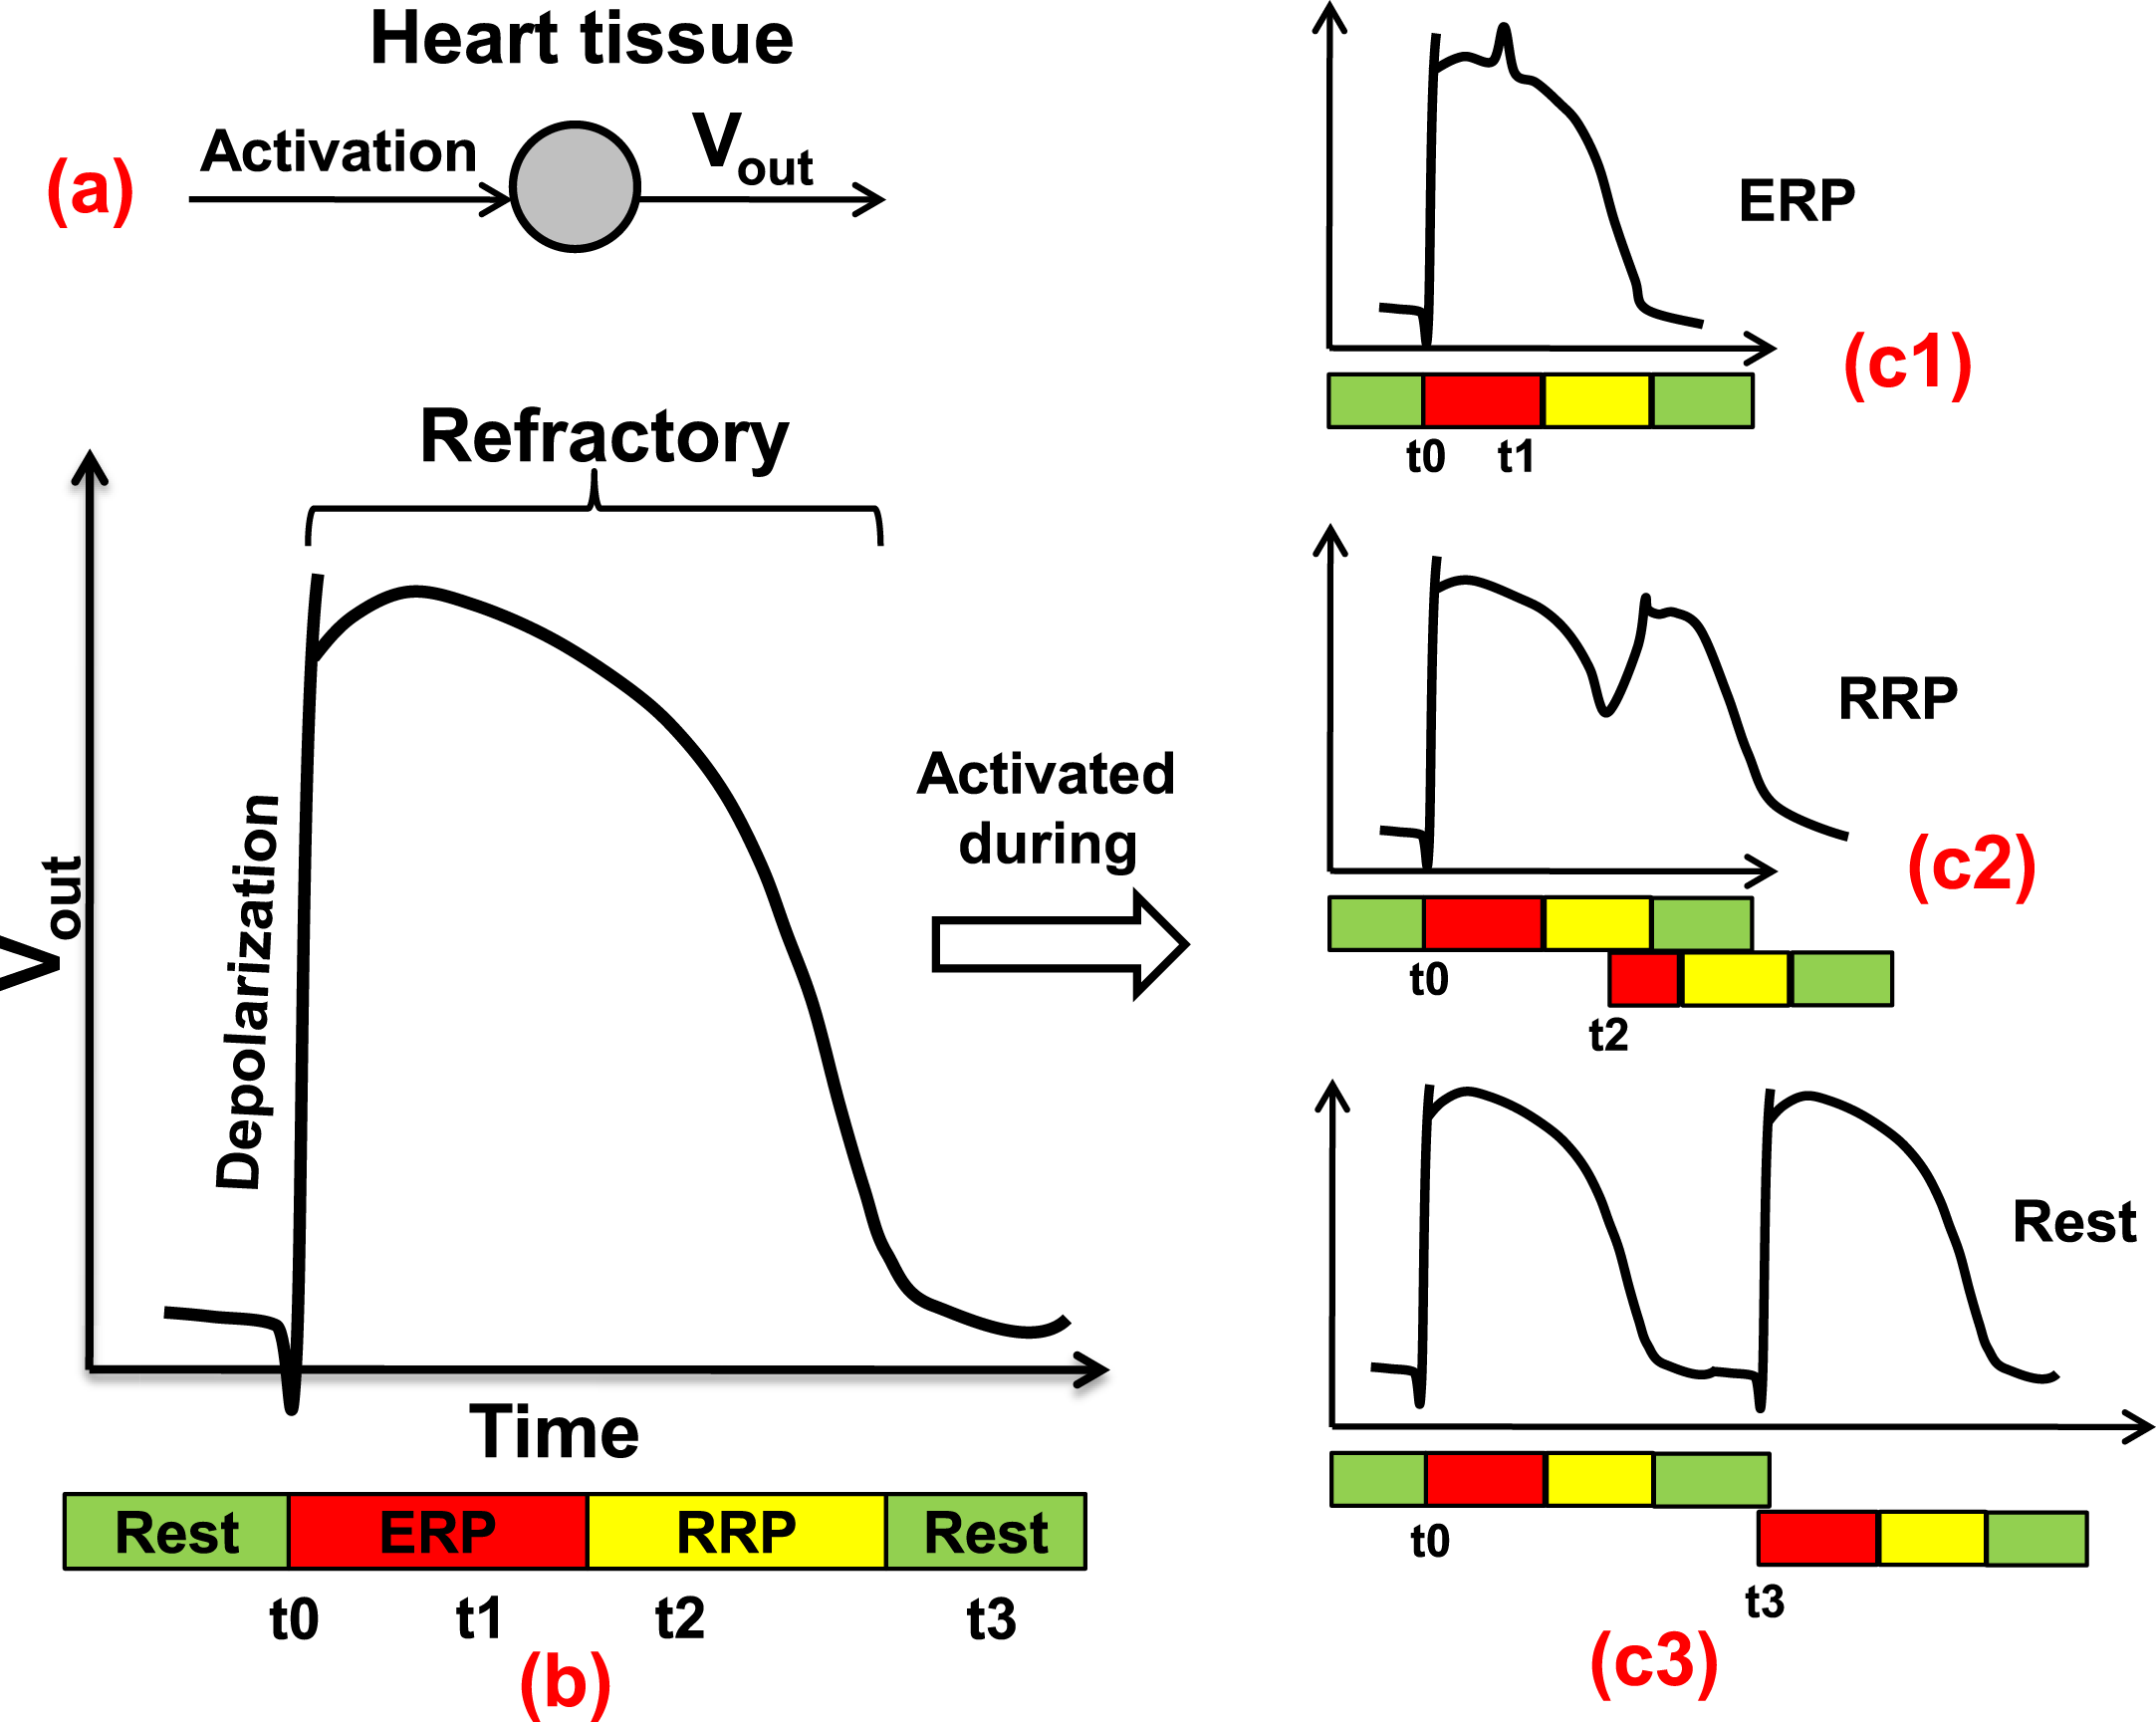
\includegraphics[width=0.7\textwidth]{figs/refractory.png}
%\vspace{-10pt}
\caption{(a) The generation of Action potential; (b) Action potential; (c1) The second activation arrived during ERP; (c2) Arrived during RRP; (c3) Arrived after refractory.}
\label{fig:refractory}
%\vspace{-10pt}
\end{figure} 
\subsection{Cellular Level ElectroPhysiology}
The contraction of heart muscles can be triggered by external voltage applied to the cell. After the activation, a transmembrane voltage change over time can be sensed due to ion channel activities, which is referred to as an Action Potential (\figref{refractory}(a)). The upstroke of the action potential is called depolarization, during which the muscle will contract. The voltage change caused by the depolarization will depolarize the cells nearby, which causes an activation wave across the heart. After the depolarization there is a refractory period during which the cell recovers to the pre-excitation state and the voltage drops down to the resting potential. The refractory period can be divided into \emph{Effective Refractory Period (ERP)} and \emph{Relative Refractory Period (RRP)} (\figref{refractory}(b)). During ERP, the cell cannot be depolarized due to the lack of the ion. As the result, the activation wave will be "blocked" at the tissue during ERP (\figref{refractory}(c1)). During RRP, the cell is partially recovered and the cell can be depolarized. However, the new action potential generated by the depolarization will have different morphology, thus affecting the refractory periods of the tissue and conduction delay of the activation wave (\figref{refractory}(c2)). \figref{refractory}(c1)-(c3) show the action potential shape change and corresponding timing change in refractory periods when the cell is activated at time stamp $t1$, $t2$, $t3$ after the initial activation $t0$. 



\subsection{Electrical conduction system of the heart}
Heart tissue with different timing parameters assemble the electrical conduction system to ensure coordinated contraction of the heart. First, specialized tissue at the Sinoatrial (SA) node periodically and spontaneously self-depolarizes. This is controlled by the nervous system and the SA node is the primary and natural pacemaker of the heart. The activation signal then travels through both atria, causing contraction and pushes blood into the ventricles. Then the activation is delayed at the Atrioventricular (AV) node which allows the ventricles to fill fully. The fast-conducting His-Purkinje system then spreads the activation signal within both the ventricles. The simultaneous contraction of the ventricle muscles will push the blood out of the heart.
%\begin{figure*}[!t]
%\centering
		%\subfigure [\small]{			
		%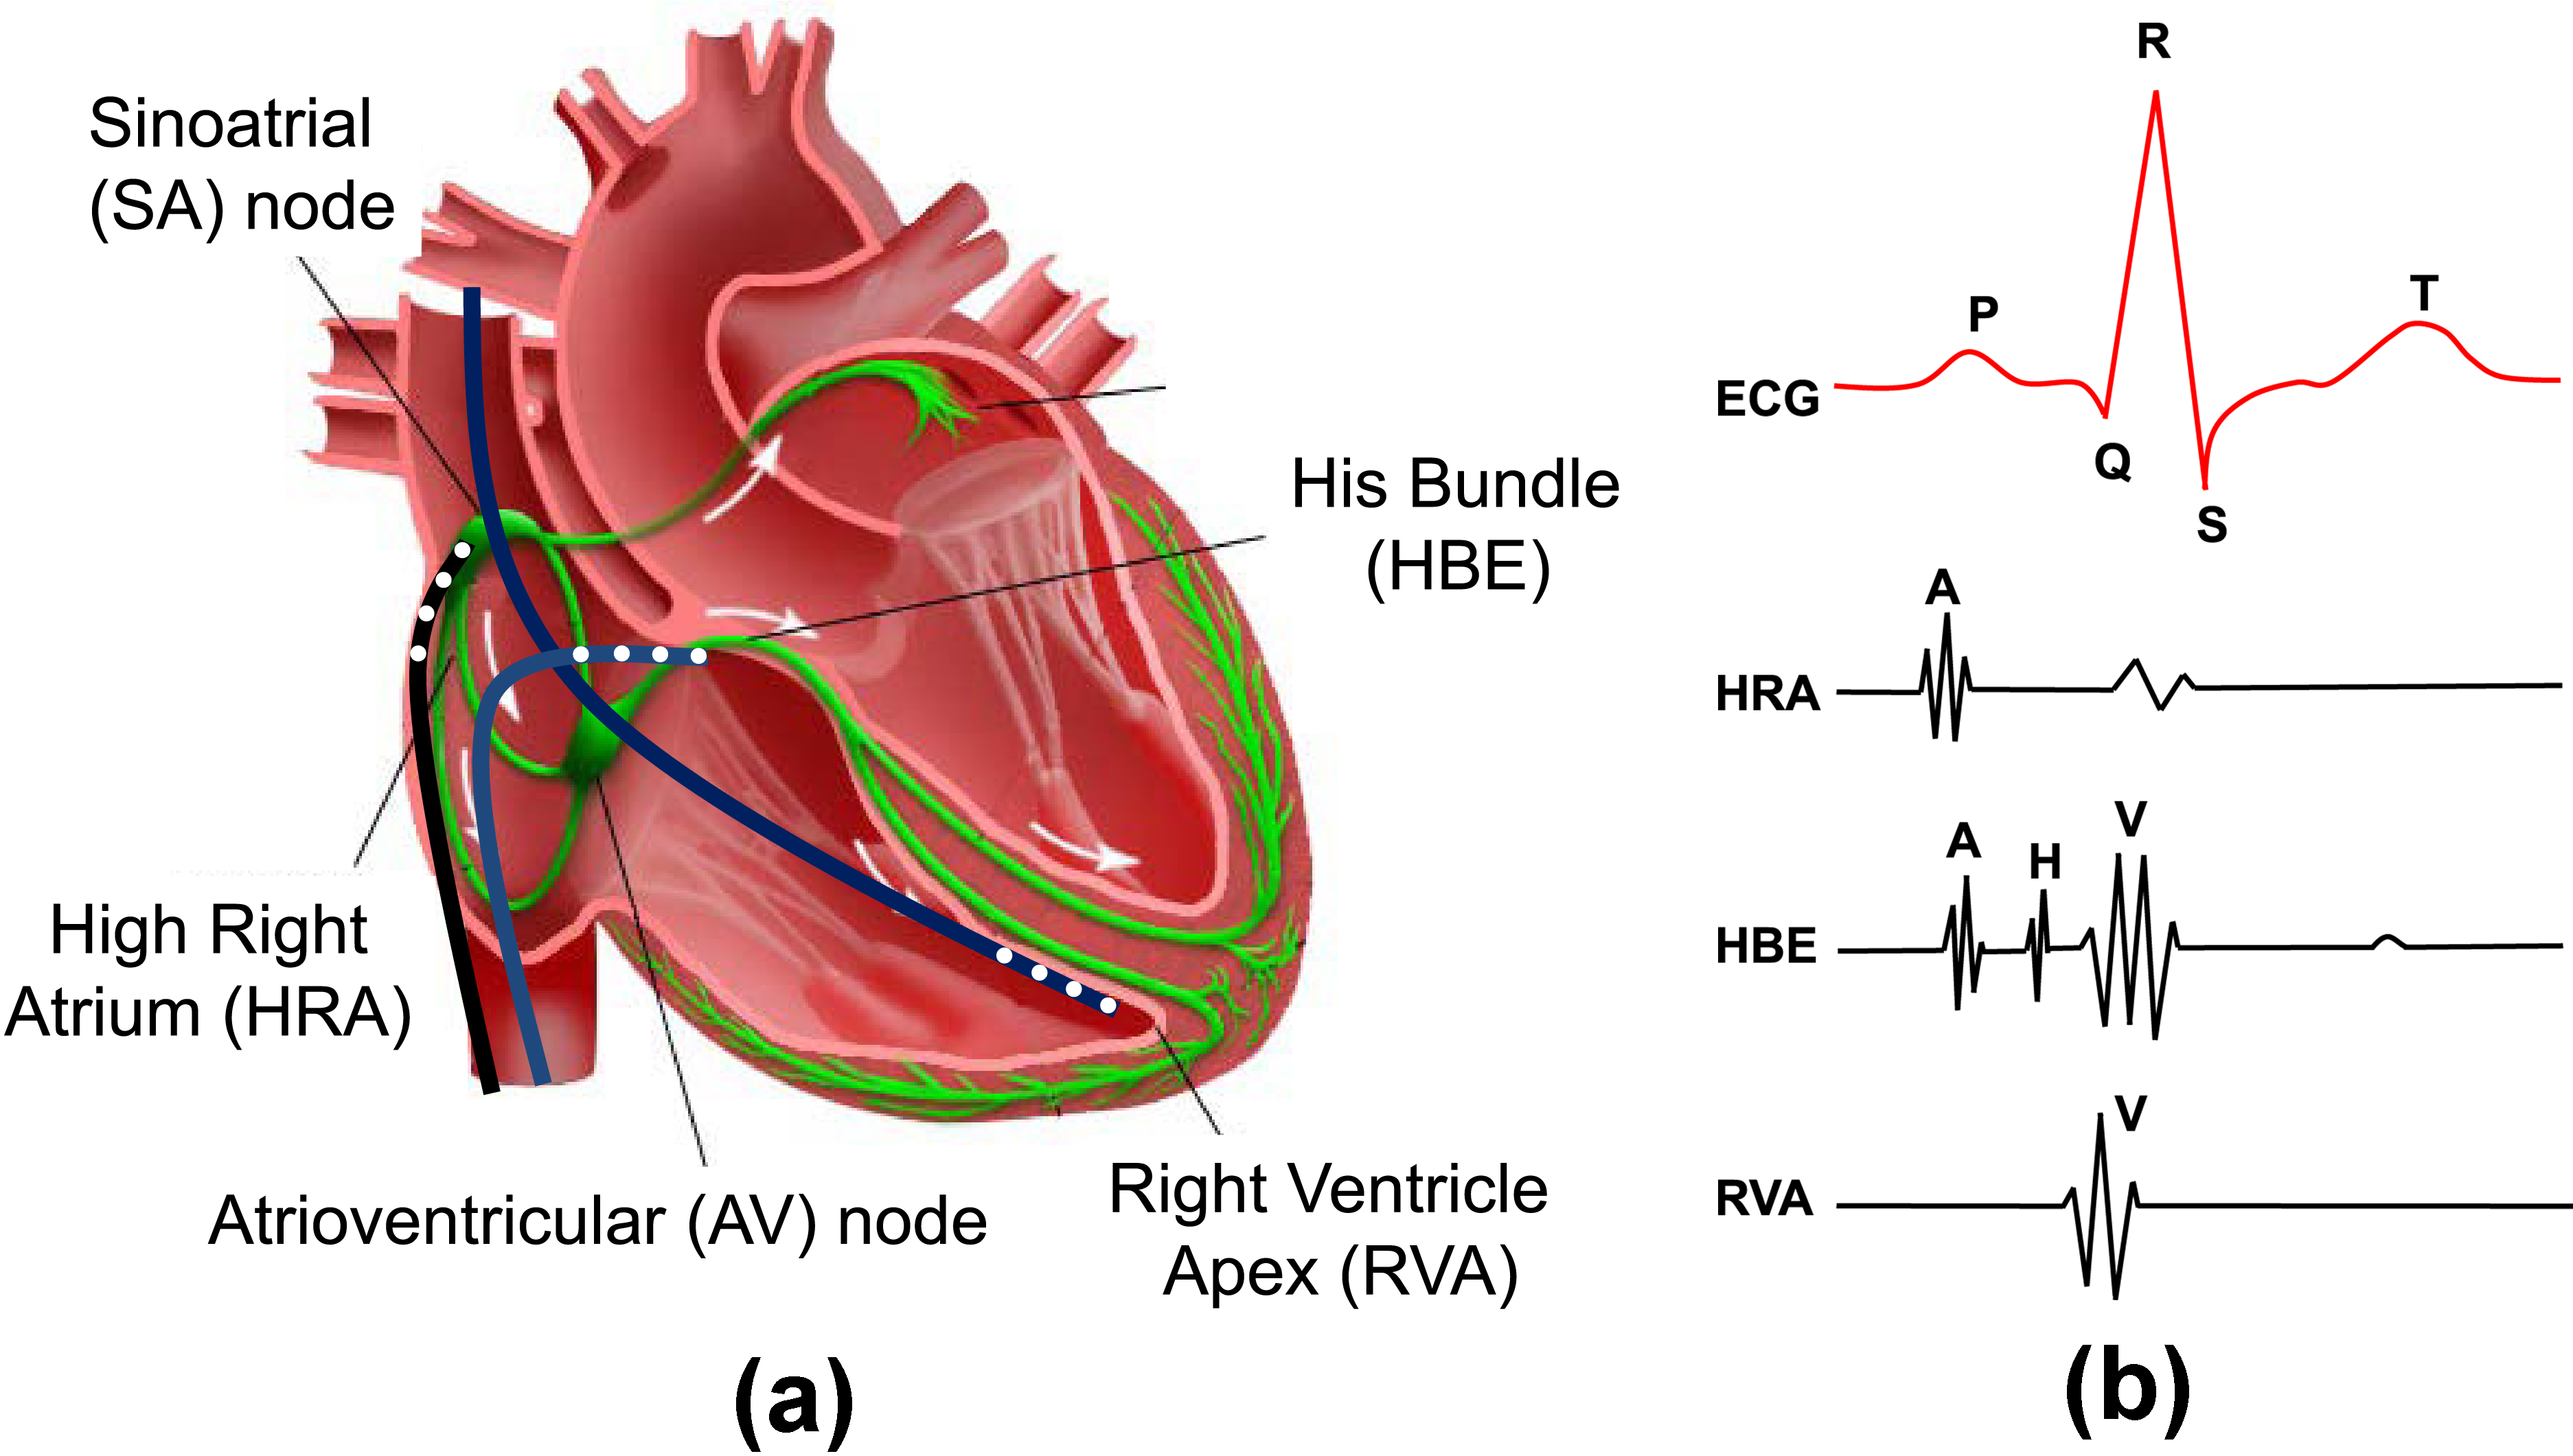
\includegraphics[width=0.3  \textwidth]{figs/probes.png}
		%\label{fig:probes}
		%} 
%
		%\subfigure [\small] 
		%{
		%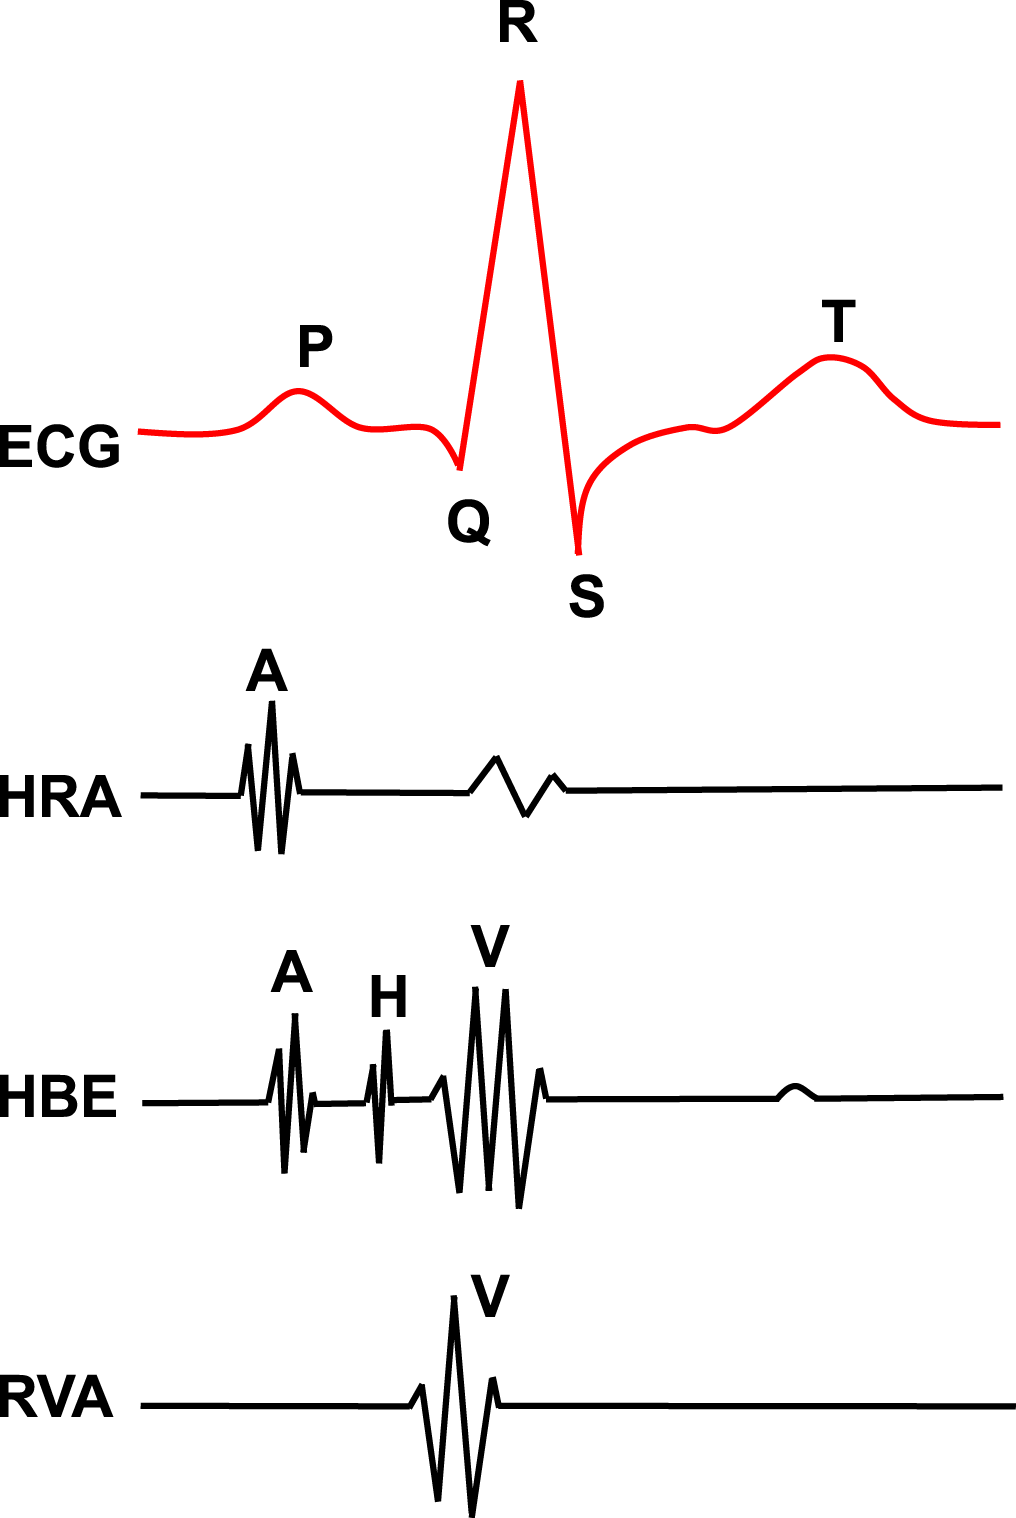
\includegraphics[width=0.2\textwidth]{figs/egm.png}
		%\label{fig:egm}
		%} 
%%\vspace{-10pt}
%\caption{\small (a) Node automaton. Dotted transition is only valid for pacemaker tissue like SA node; (b) Path automaton; (c) Model of the electrical conduction system of the heart using a network of node \& path automata~\cite{vhm_ecrts10}.}
%%\vspace{-15pt}
%\end{figure*} 

%\section{Electrophysiological Testing}
\Hao{A figure for heart and pacemaker}

%\chapter{Modeling the Physiological Environment}
%\begin{itemize}
	%\item How to encode domain knowledge of the physiological environment into models?
    %\item What are the applications that the models will be used?
    %\item What are the differences in terms of environment models between model checking and simulation?
    %\item How to balance complexity and expressiveness of the model?
%\end{itemize}

%In the following sections, we demonstrate how to construct heart models for closed-loop verification of implantable pacemaker. Note that for two different applications the models are constructed differently as we address their respective requirements for environment models. 


\section{Heart Models For Closed-loop Testing}
%\begin{itemize}
	%\item Why the models at this level have to be deterministic? Where can they be used?
    %\item How electrophysiology reflects the functions of the heart?
    %\item How to encode these knowledge into models?
    %\item Why VHM has the right level of details for pacemaker verification?
    %\item How VHM interacts with pacemaker?
    %
%\end{itemize}
During closed-loop testing, the devices interact with the environment (or its models) under different environmental conditions. The closed-loop executions are monitored and violations of safety/efficacy requirements are reported. In model-based closed-loop testing, the environment models are expected to mimic the behaviors of actual environment and its interaction with the device. Thus the environment models are in general deterministic so that the execution traces are reproducible. Complex dynamics during state transitions also need to be captured to validate violations within longer executions traces. 

\subsection{Modeling Philosophy}

\textbf{Interface to the device: }The pacemaker can only sense and actuate from two locations within the heart, the spatial fidelity requirement for the heart model is thus low. The diagnosis of heart conditions only relies on the timing of the electrical events, thus the behaviors of the model can be reduced to timing only, if a temporal model of the heart is rich enough to represent majority of heart conditions. \\
\textbf{Model expressiveness: }Electrophysiology (EP) is an active field in cardiology based on the fact that the mechanical functions of the heart are largely correlated with the electrical activities. During an EP testing procedure, the physicians diagnose heart conditions by examining the patterns and intervals of local electrical activations (temporal) measured from electrodes placed into different locations of the heart (spatial). 

Based on the analysis above, an EP-based spatial and temporal model of the heart is capable of representing the electrical behaviors of different heart conditions, and more importantly, their interaction with a pacemaker. 

\subsection{Heart Model Components}
We introduce the model components that can be used to configure heart models corresponding to different heart conditions. As introduced in Chapter 2, the action potential of a heart tissue has 3 timing periods during which the tissue responds to external electrical stimuli differently. We use an extended timed-automata formulation (\cite{timed_automata}) to model the timing behaviors of a heart tissue during each cycle. We refer the tissue model as \emph{Node automaton} and \figref{node_automata} shows the structure of a node automaton $i$. 3 states correspond to 3 timing periods of the action potential. From \textsf{Rest} state, the node can either self activate or activated by external stimuli (Act\_node) and go to \textsf{ERP} state. During \textsf{ERP} state the node does not respond to external stimuli (blocked). During \textsf{RRP} state, the node can still be activated and go to \textsf{ERP} state, however the ERP period and the conduction delay of the tissue are affected by the "earliness" of the activation arrived during the RRP period, which is tracked by a shared variable $C(i)$. The new ERP period is determined by a function over clock value $g(f(t))$ which mimic the beat-to-beat dynamics described in \cite{josephson}. The function $g$ and $f$ are given by:
\begin{equation} \label{factor}
						f(t) = 1-t/Trrp
						\end{equation}
and
%  The AV node has a different profile than the other tissue. The ERP period increases rather than decreases when activated during its RRP (~\cite{josephson}).
\begin{equation} \label{earliness_noAV}
						g(x) = \left\{
						\begin{array}{lr}
						
						T_{min}+(1-(1-x)^3)\cdot (T_{max}-T_{min}), i=AV\\
						T_{min}+(1-x^3)\cdot (T_{max}-T_{min}),i\neq AV
			
						
						\end{array}
						\right.
						\end{equation}  
where $T_{min}$ and $T_{max}$ are the minimum and maximum value for \emph{Terp} of the tissue.
\begin{figure*}[!t]
\centering
		\subfigure [\small]{			
		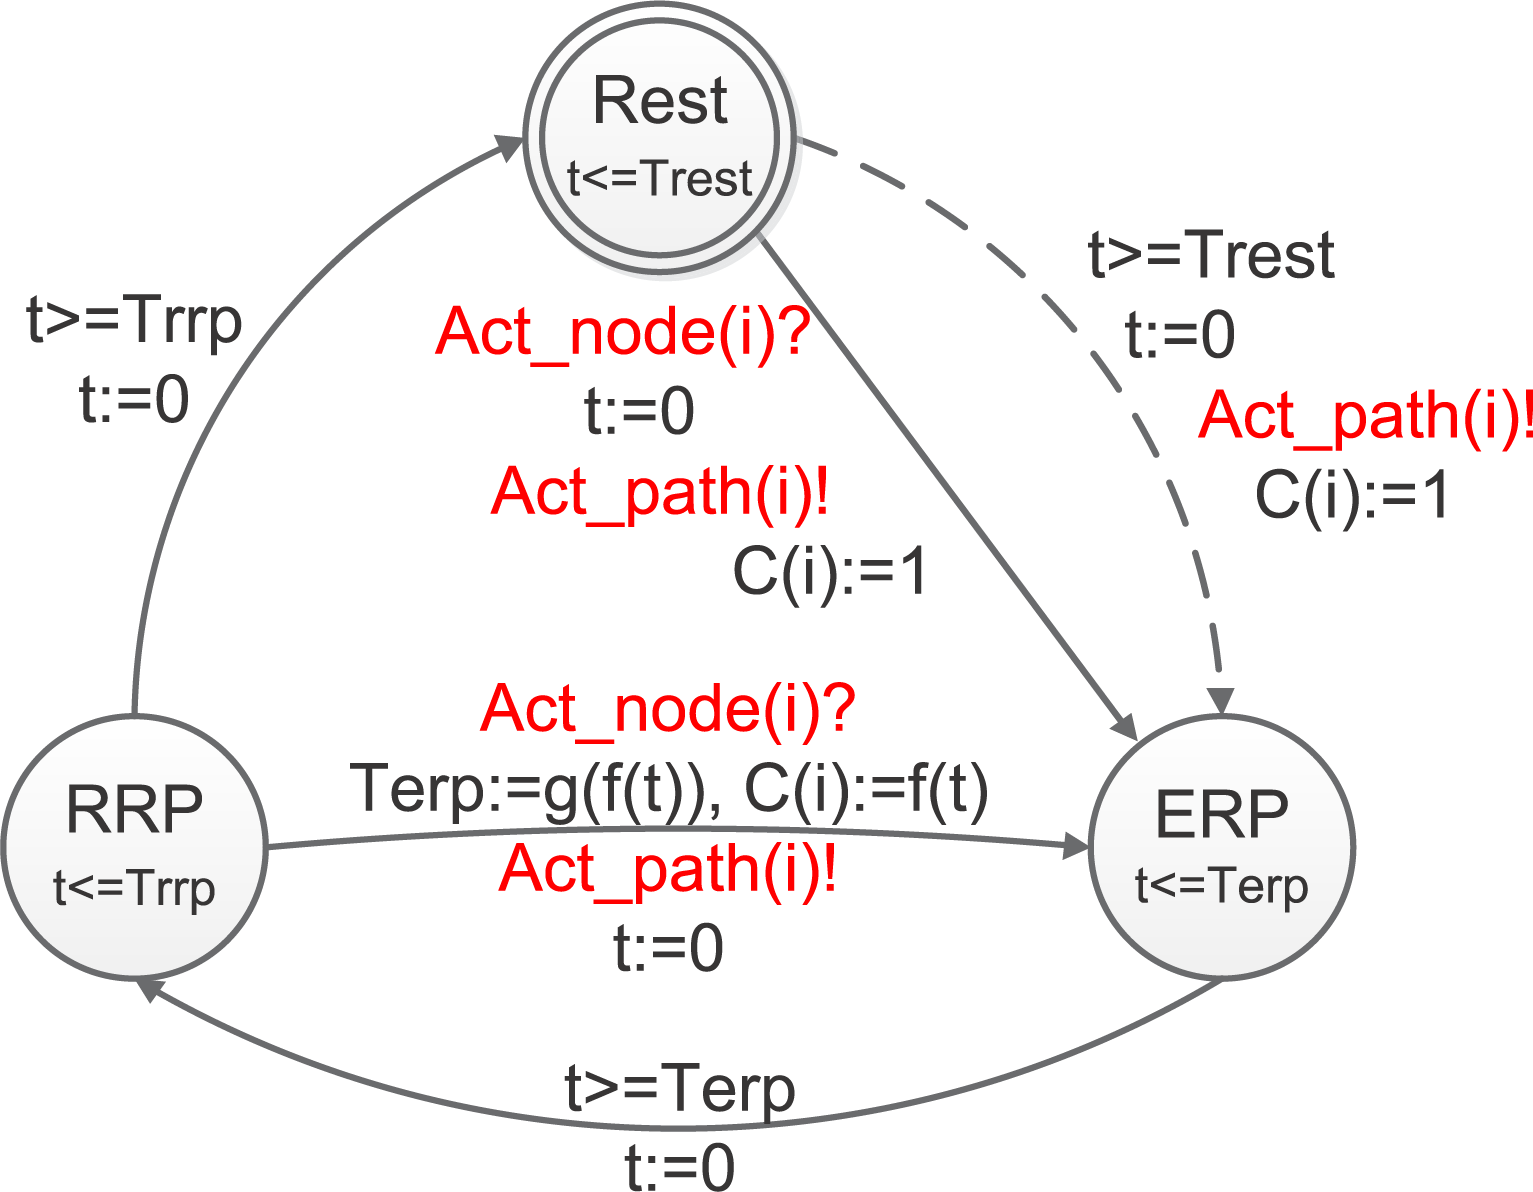
\includegraphics[width=0.35\textwidth]{figs/node_aut.png}
		\label{fig:node_automata}
		} 
%	\hspace{.1in}%
		\subfigure [\small] 
		{
		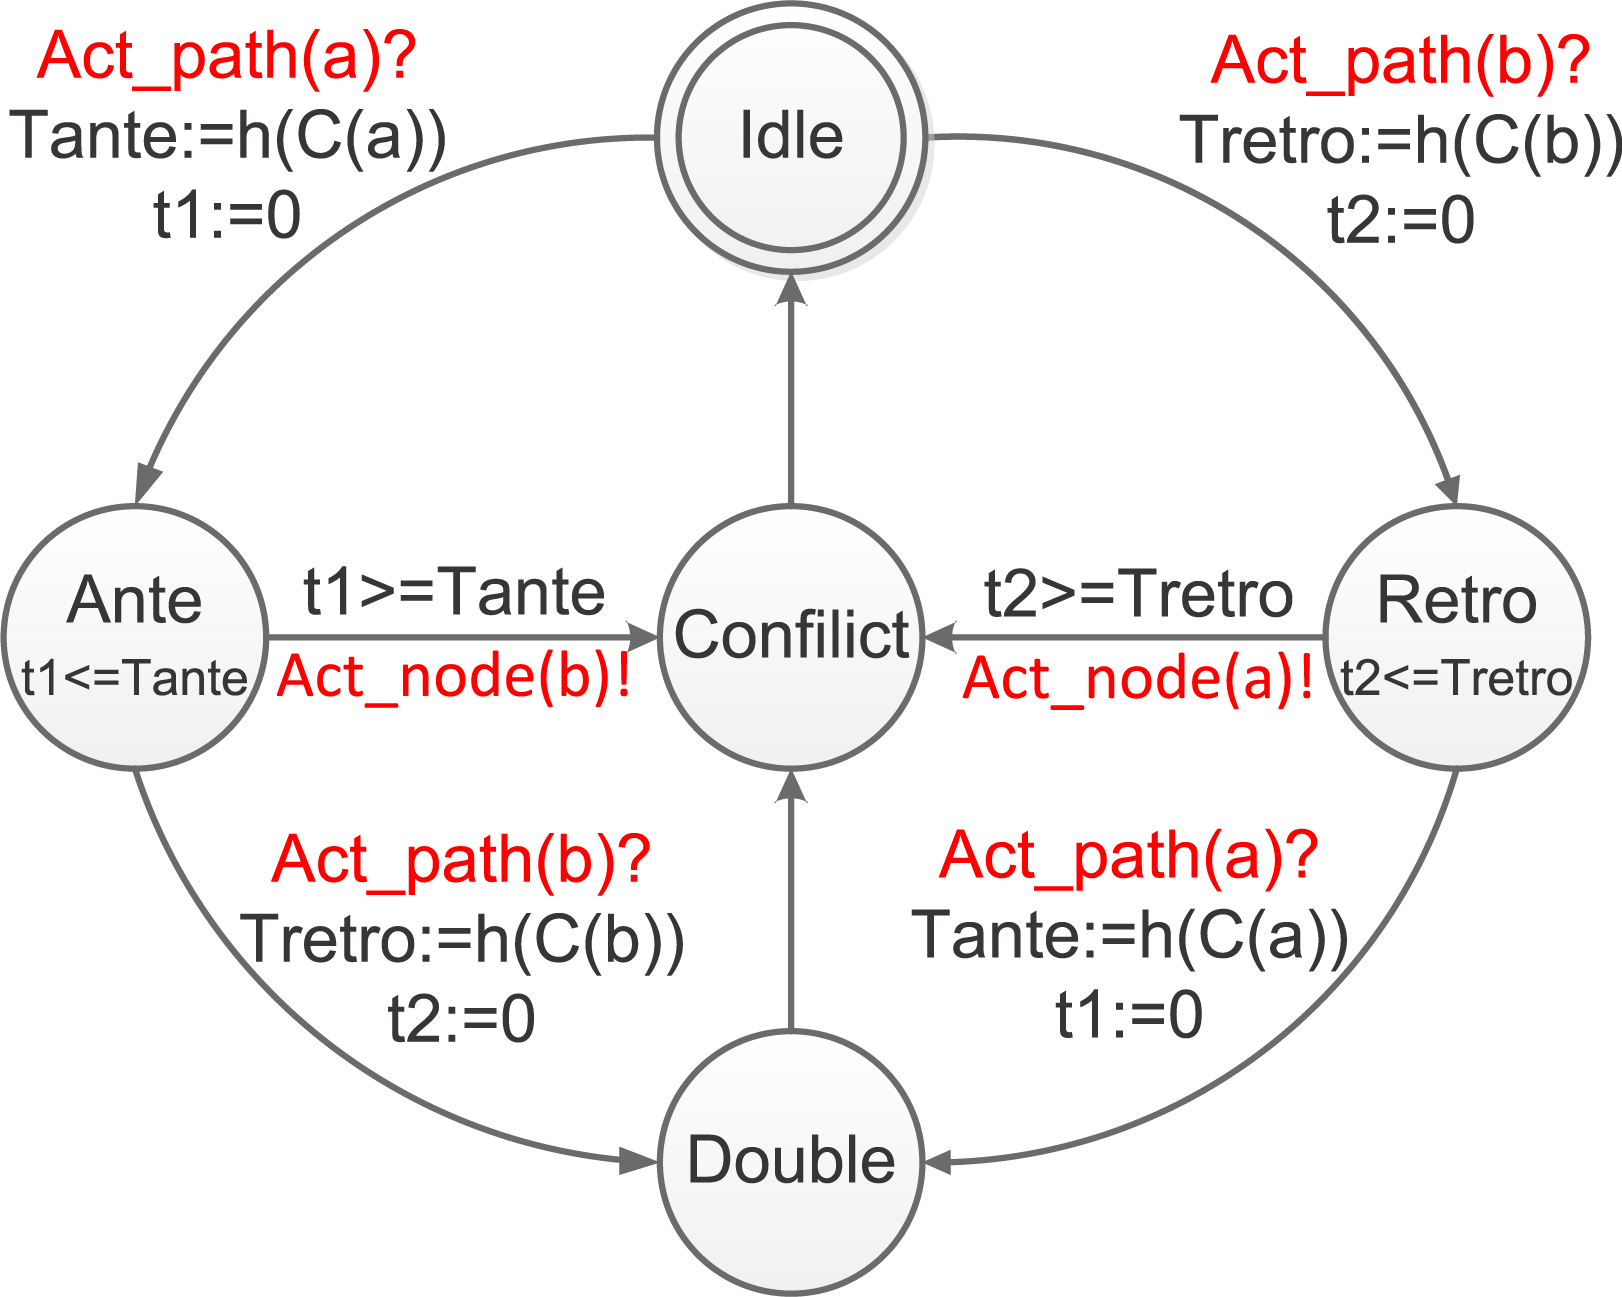
\includegraphics[width=0.35\textwidth]{figs/path_aut.png}
		\label{fig:path_automata}
		} 
		\subfigure [\small] 
		{
		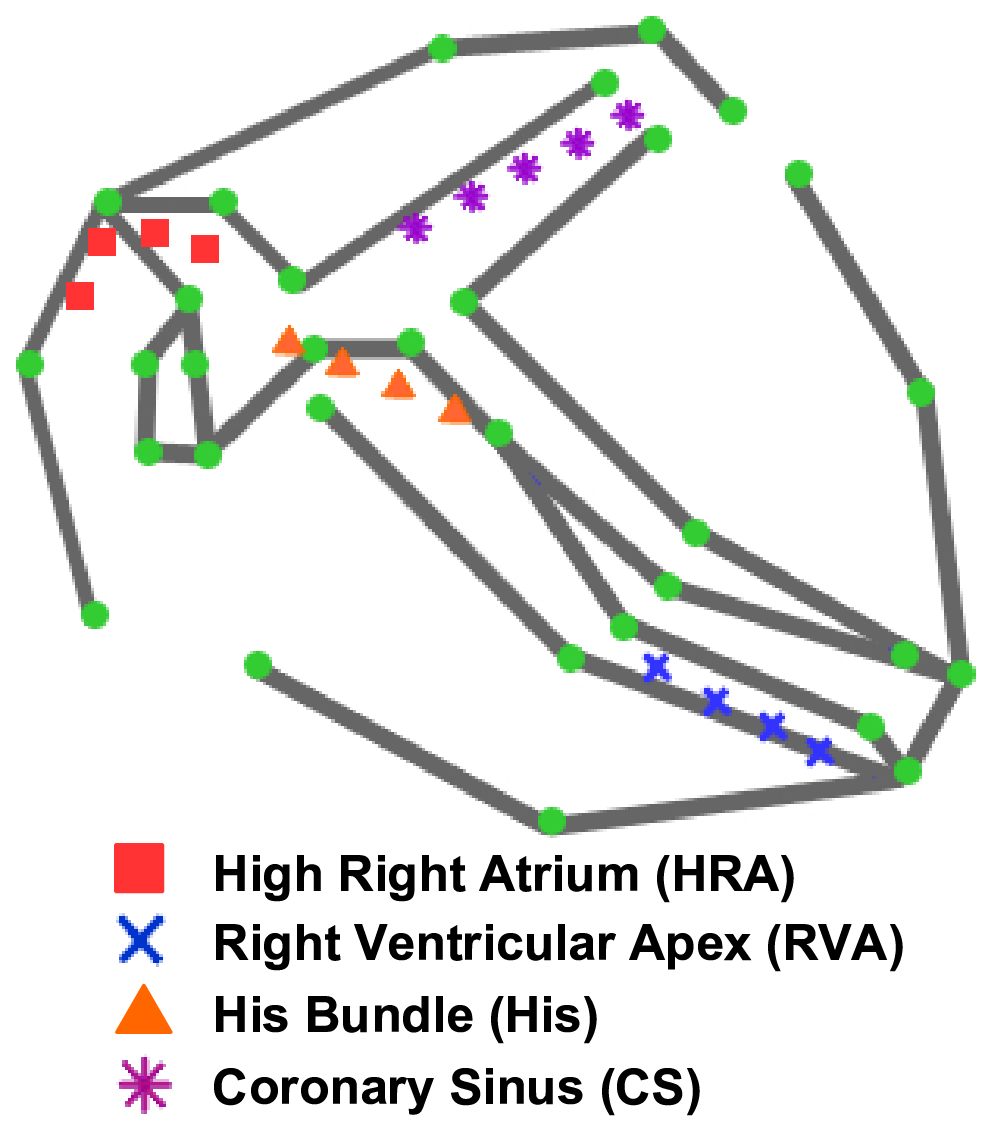
\includegraphics[width=0.2\textwidth]{figs/gen_setup.png}
		\label{fig:general_setup}
		} 
\label{fig:h_automatas}
%\vspace{-10pt}
\caption{\small (a) Node automaton. Dotted transition is only valid for pacemaker tissue like SA node; (b) Path automaton; (c) Model of the electrical conduction system of the heart using a network of node \& path automata ~\cite{vhm_ecrts10}.}
%\vspace{-15pt}
\end{figure*} 

Due to the limited number of observable points within the heart, modeling every tissue of the heart and its full anatomy is unnecessary and unfeasible. In our heart models, only self-activating tissue and key hubs of the electrical conduction system are modeled as node automata. The electrical conduction through the tissue between nodes are abstracted using \emph{path automata}. The path automata can be used to represent structural or topological (functional) electrical connections between nodes. \figref{path_automata} shows a path automaton connecting node a and b.

The initial state of a path automaton is \emph{Idle}, which corresponds to no conduction. The states corresponding to the two conduction directions are named after the physiological terms: Antegrade (Ante) and Retrograde (Retro). These states can be intuitively described as forward and backward conductions. If \emph{Act\_path} event is received from one of the nodes connected to it, the a transition to \emph{Ante} or \emph{Retro} state correspondingly will occur in the path automaton. At the same time the clock invariant of the state is modified according to the shared variable \emph{C(a/b)}. This corresponds to the change of the conduction delay that is caused by the early activation. Similar to node automaton, the changing trend is extracted from clinical data and the function $h$ is defined as:
\begin{equation} 
						h(c) = \left\{
						\begin{array}{lr}
						
						path\_len/v\cdot (1+3c), i=AV\\
						path\_len/v\cdot (1+3c^2), i\neq AV
						\end{array}
						\right.
						\end{equation}
where $path\_len$ denotes the length of the path and $v$ is the conduction velocity.

After \emph{Tante} or \emph{Tretro} time expires, the path automaton sends out \emph{Act\_node(b)} or \emph{Act\_node(a)} respectively. A transition to \emph{Conflict} state occurs followed by the transition to \emph{Idle} state. The intermediate state \emph{Conflict} is designed to prevent back-flow, where the path is activated by the node \emph{b} it has just activated. If during \emph{Ante} or \emph{Retro} state another \emph{Act\_path} event is received from the other node connected to the path automaton, a transition to \emph{Double} state will occur, corresponding to the two-way conduction. In this case, the activation signals eventually cancel each other and the transition to \emph{Idle} state is taken.

\subsection{Modeling the Electrical Conduction System}
The node and path automata are the basic components for heart modeling. Different hearts under different conditions have different timing parameters and/or different conduction topology. We connect node and path automata with different timing parameters into a network to represent different heart conditions. (\figref{general_setup}) 

\subsection{Interaction With The Heart Model}
In EP testing and pacemaker application, the local electrical activities, measured as electrogram (EGM) signals, are used to diagnose heart conditions. During heart model construction, we can assign a node automaton at electrode locations and the transitions to the ERP state can be used to represent the local activation events. In a more general setup where electrodes are assigned anywhere within the heart model, a probe model is designed to generate synthetic EGM signals using temporal information and spatial information from the network of node and path automata. \figref{egm_s} shows the morphology of EGM signal changes with different conduction velocity and probe configurations. Due to space limitation, detailed description of the probe model can be found in \cite{vhm_embc11}.

\begin{figure}[!t]
\center
%\vspace{-15pt}
		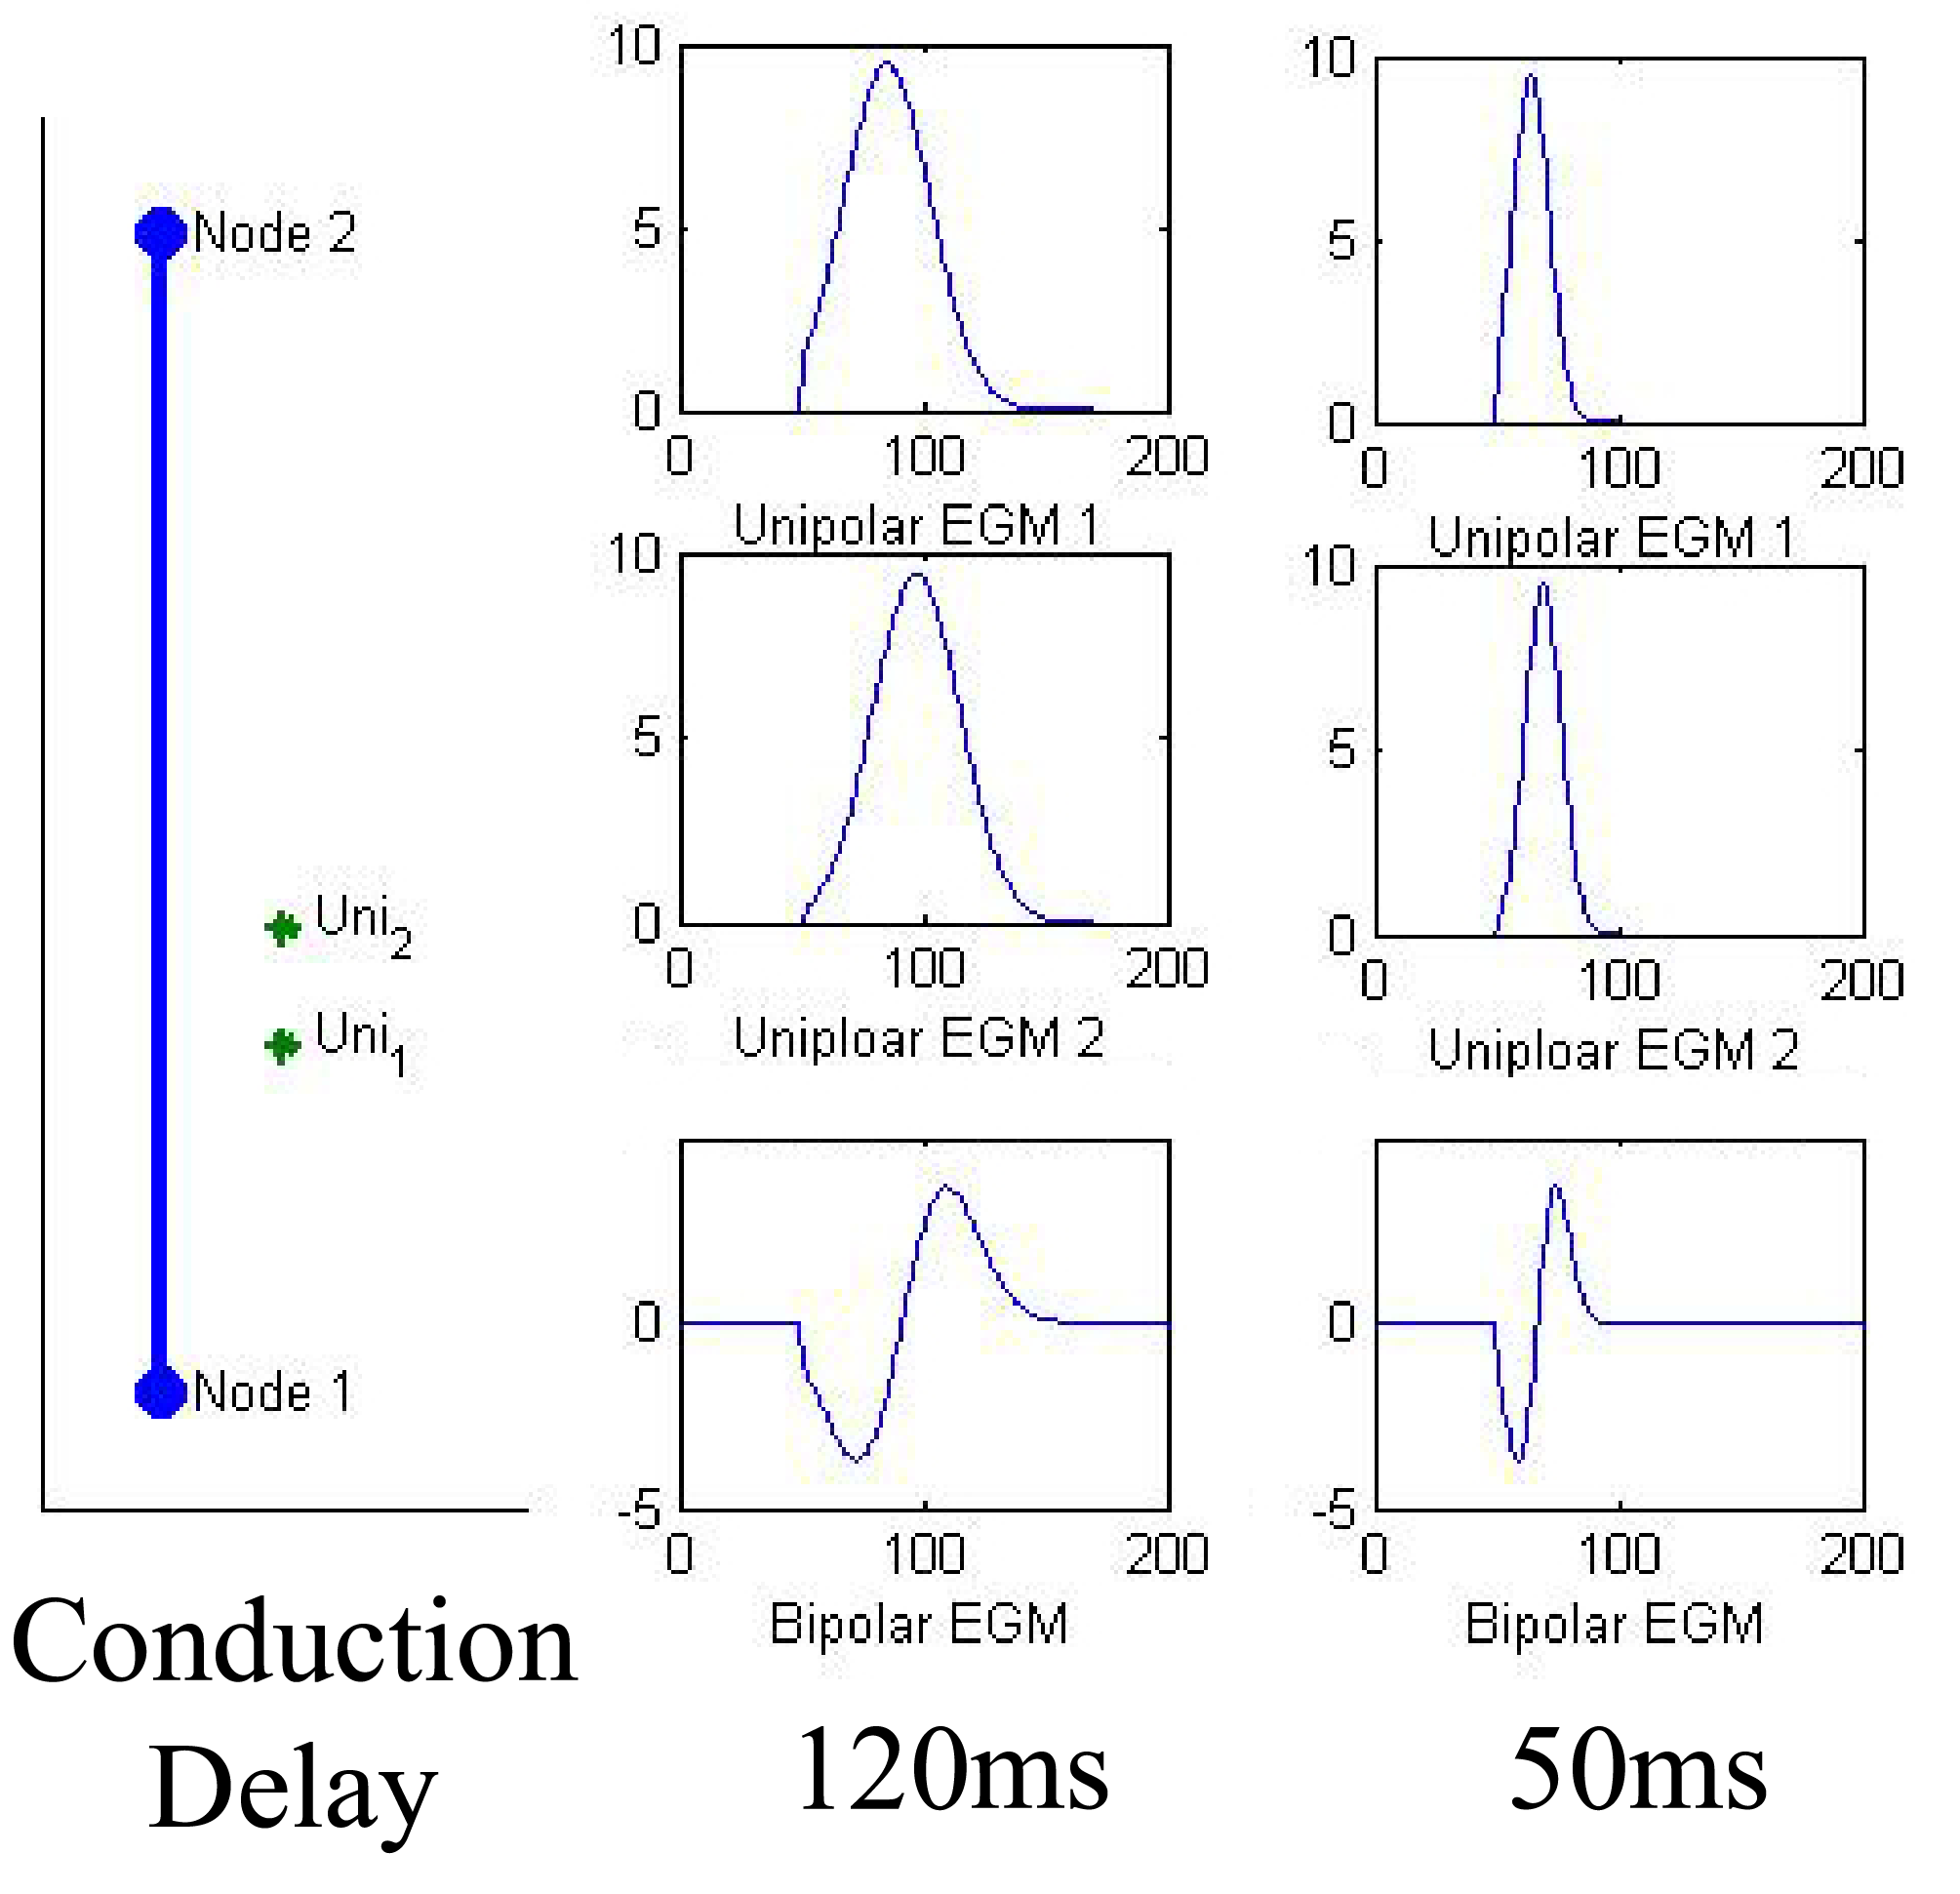
\includegraphics[width=0.45\textwidth]{figs/fig7.png}
%\vspace{-10pt}
\caption{The influence of conduction velocity and probe configuration on the EGM morphology. The left columns show the placement of probes in relation to the path; the right columns show the functional EGM.}
\label{fig:egm_s}
%\vspace{-15pt}
\end{figure}

\section{Non-deterministic Models for Closed-loop Model Checking}
%\begin{itemize}
	%\item What does nondeterminism do? Where can these model be used?
    %\item How to replace complex dynamics of the deterministic models with nondeterminism?
    %\item What are the abstraction rules that can be applied to the heart models and what are their physiological basis?
    %\item How to encode the information loss during each abstraction steps?
%\end{itemize}
During closed-loop model checking, the whole closed-loop state space of the device and the environment is mathematically explored against physiological requirements. The  ideal environment models should be: 1) simple enough to avoid the state space explosion problem, 2) general enough to cover possible physiological conditions, 3) complex enough to represent any specific physiological conditions. It is obvious that no single model can achieve all 3 properties. A rigorous framework should be adapted so that appropriate models are selected for corresponding requirement.
\subsection{Modeling Philosophy}
\textbf{Model Formalism: }Choosing an appropriate formalism for the physiological models is important as the formalism determines the closed-loop state space and the feasibility/efficiency to do model checking. Pacemaker utilize the timing of local electrical events to diagnose heart conditions. It is therefore intuitive to use timed-automata models of the heart. Timed-automata is also compatible with model checking tools like UPPAAL (\cite{uppaal_tut}) so that the whole closed-loop state space can be explored.\\
\textbf{Model Coverage: }Pacemakers are designed to treat bradycardia, however not only should the pacemakers maintain appropriate heart rate when the intrinsic rate is low, but also shall not degenerate other heart conditions. Even for the same patient the condition also changes over time that has to be taken into account. In order to achieve safety across all possible heart conditions, the heart models used during closed-loop verification should be able to cover all possible heart behaviors, more precisely, their mapping to pacemaker inputs. Over-approximation (\cite{CEGAR}) with non-determinism can be used to simplify model structure while covering larger variety of environmental behaviors. Techniques like model-checking can then be used to examine the whole closed-loop state space for property violations.\\ 
\textbf{Ambiguity Due To Low Sensing Capability: }The sensing resolution of pacemakers is low, in terms of the number of sensing location (2 leads), as well as the information obtained from each sensing location (binary events). If abstraction rules utilize the fact that different heart conditions may generate exactly the same input sequence to the pacemaker, there will be ambiguities on concretizing abstract closed-loop executions. For certain conditional requirements, it is important to differentiate all possible concrete executions corresponding to an abstract execution. As the result, the heart model(s) should have the capability to differentiate these heart conditions when verifying certain properties.\\
\textbf{Information Lose During Abstraction: }While over-approximation achieves simplicity and coverage, it also inevitably introduces invalid behaviors into the model which can cause false-negatives and false-positives during model checking. To solve this problem, more refined models of the heart should be available which can differentiate and eliminate invalid executions when necessary to avoid false-positives.

The most challenging aspect during closed-loop model checking is environment model abstraction and refinement. In \cite{STTT13} we developed a series of heart model abstractions at various abstraction levels. The models are abstracted using abstraction rules derived from physiological knowledge, thus ensuring that each abstraction step covers more physiological conditions. The models in adjacent abstraction levels also satisfy \textsf{timed-simulation} relationship (\cite{simulation}) to ensure complete coverage in the more abstract model. In the rest of the section, we briefly discuss the modeling process and the domain knowledge used. The detailed abstraction and proof for simulation relationship can be found in \cite{STTT13}.
\begin{figure}[!t]
\center
%\vspace{-10pt}
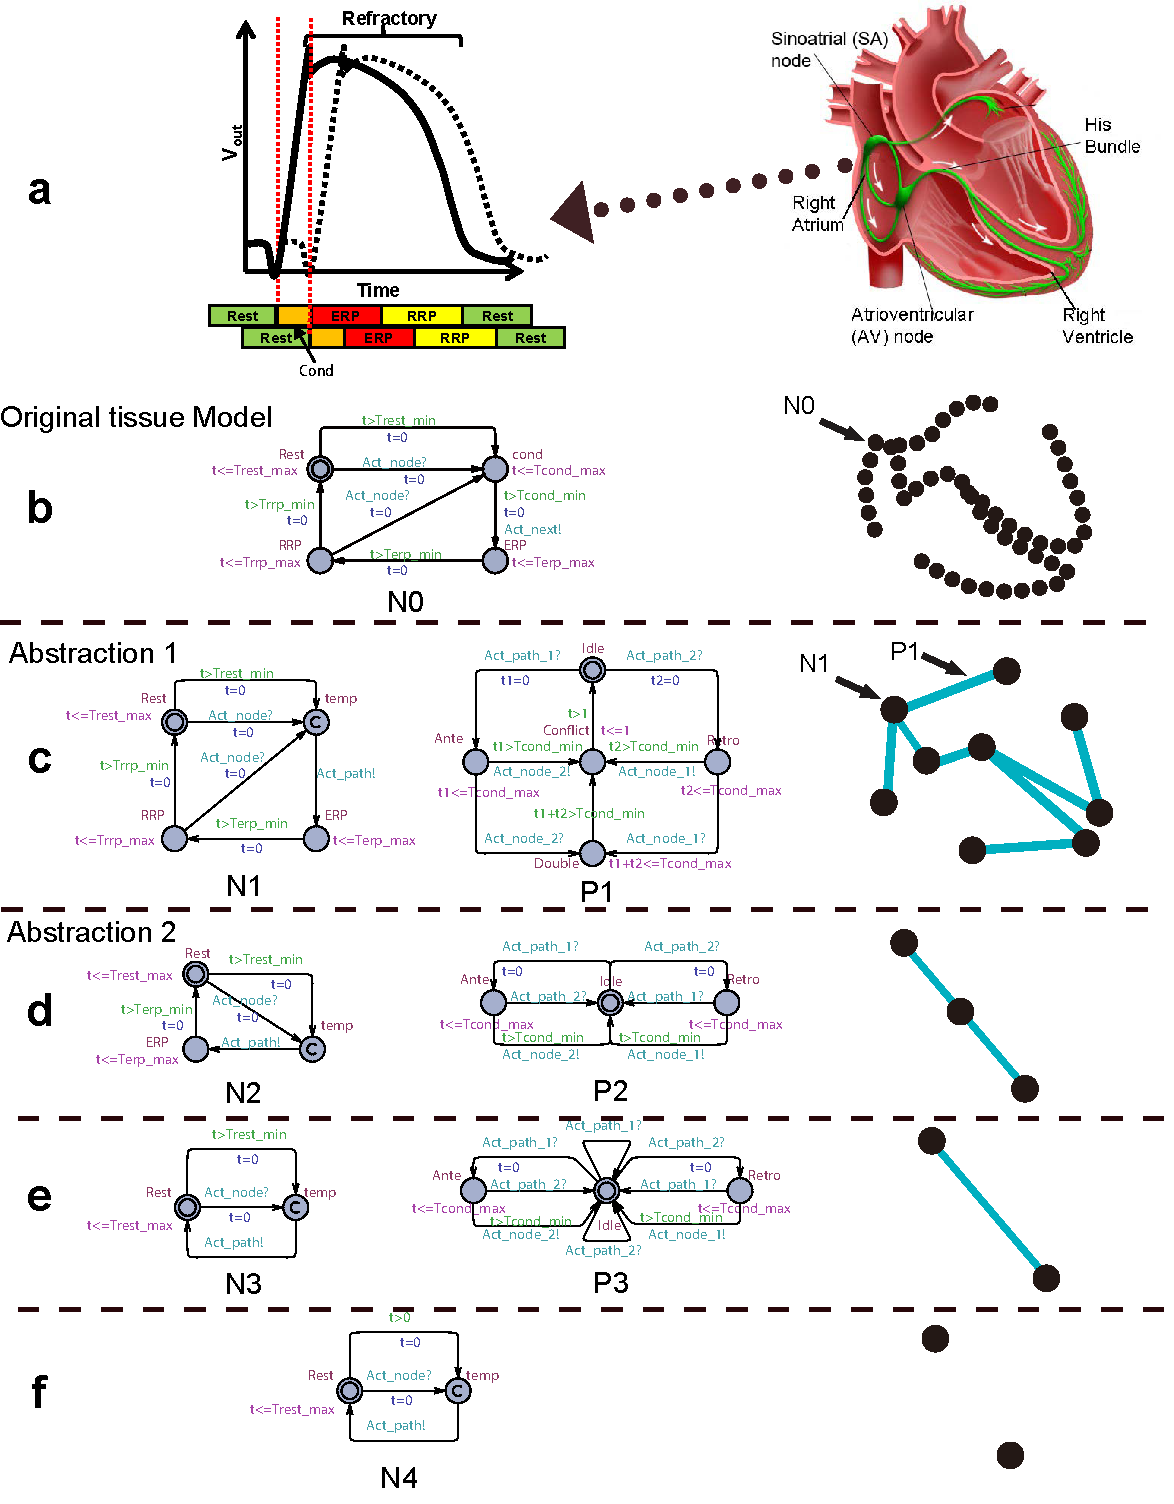
\includegraphics[width=0.9\textwidth]{figs/Heart_abs.pdf}
%\vspace{-10pt}
\caption{(a) The generation of Action potential; (b) Action potential; (c1) The second activation arrived during ERP; (c2) Arrived during RRP; (c3) Arrived after refractory. (\cite{STTT13})}
\label{fig:HM_abs}
%\vspace{-10pt}
\end{figure} 
\subsection{Initial Abstraction}
For the initial heart model, spatially we assume that every heart tissue are modeled. Temporally we model each heart tissue as an automaton $N0$ shown in \figref{HM_abs}.b. The beat-to-beat dynamics of heart tissue discussed in the last section is abstracted using non-determinism, as the ERP period and conduction delay of the tissue are non-deterministically chosen from ranges instead of deterministic functions. The model covers all possible timing behaviors of a heart tissue. 

\subsection{Abstract Conduction Delays With Paths}
At the first abstraction step, we seperate the conduction delay (modeled by the cond state in $N0$) from the new node automata $N1$ and model the conduction between two nodes using path automaton $P1$. Since the beat-to-beat dynamics are abstracted with non-determinism, the RRP state is merged with the Rest state in $N1$. 

we only model the following kinds of heart tissue with node automata and abstract other heart tissue with path automata:
\begin{itemize}
	\item Self-depolarizing tissue
    \item Tissue with long ERP period
    \item Tissue forming conduction loops
\end{itemize}

\subsection{Merging}
abstract heart tissue
% \subsubsection{Abstracting Beat-to-beat Dynamics}
% \subsubsection{Abstracting Conduction Delays with Path}
% \subsubsection{Merging Activation-generating Nodes}
% \subsubsection{Replace ERP Blocking With Non-deterministic Conduction}
% \subsubsection{Replace }

